\documentclass[10pt,twocolumn,letterpaper]{article}
\usepackage{cvpr}
\usepackage{times}
\usepackage{graphicx}
\usepackage{amsmath}
\usepackage{amssymb}
\usepackage[pagebackref=true,breaklinks=true,colorlinks,bookmarks=false]{hyperref}

\def\GroupID{XX} % <------- ENTER YOUR COMP6321 group number here

\begin{document}
\title{Project Title Here}
\author{Name 1 \and Name 2 \and Name 3\\(if applicable) \and Name 4\\(if applicable)}
\maketitle

\begin{abstract}
   Abstract here.
\end{abstract}

%------------------------------------------------------------------------
\section{Introduction}

This is an empty template, with a suggested top-level structure.
Custom projects should have a related work subsection and should
cite related research papers from the project's field.

%------------------------------------------------------------------------
\section{Methodology \& Experimental Results}



%------------------------------------------------------------------------
\section{Conclusions}



\appendix


%-------------------------------------------------------------------------
\section{Overview of project code and data}

% DELETE THIS TEXT
{\em Optional section.} This is a guide written by you to help the course staff.
Here you can make a few brief comments to the course staff about where
they should start when looking at your project code, *e.g.* how to run your scripts and what
data files contain the experimental results you used to draw your conclusions.
If your project code already has such information in an obvious place, such as a `README.md`
then this section is not necessary.

%-------------------------------------------------------------------------
\section{Examples of \LaTeX}

% The 'dilde' in Table~\ref{} puts a no-break space prevents "Table" and "1" so that
% the table number does not get split onto a separate line.
% and it is good LaTeX practice to put tildes between 

% DELETE THIS TEXT
This section contains some examples of \LaTeX~to help you get started.
(You should delete this section in the final report.)
This is a reference to Table~\ref{first_table} and Table~\ref{second_table}.
This is a reference to Figure~\ref{first_figure} and Figure~\ref{second_figure}.
This is a citation \cite{breiman2001statistical} and this is
multiple citations \cite{breiman2001statistical,bishop2006pattern}.
This is \textit{italics} and \textbf{bold} text.
This is a formula $\sum_{i=1}^N (y_i - \hat{y}_i(\mathbf{x}))^2$
that is inline with the text (`text style') and this is a
formula that is displayed separately (`display style'):
$$
\sum_{i=1}^N (y_i - \hat{y}_i(\mathbf{x}))^2
$$
These are formulas with an associated equation number
\begin{align}
   \mathbf{x} = \begin{bmatrix}
      x_1, x_2, \ldots, x_N
   \end{bmatrix}^T    \label{xvec}\\
   \boldsymbol{\phi} = \begin{bmatrix}
      \phi_1, \phi_2, \ldots, \phi_M
   \end{bmatrix}^T    \label{phivec}
\end{align}
and we can now refer back to~\eqref{xvec} or to ~\eqref{phivec} like so.



% DELETE THIS TABLE
\begin{table}
   \begin{center}
   \begin{tabular}{|l|c|c|}
   \hline
   Method & Ultra-Clustering & Random Jungles \\
   \hline\hline
   Theirs & Works OK & All your base\\
   Yours & Works better & are belong to us!\\
   Ours & Works best! & I can haz publication?\\
   \hline
   \end{tabular}
   \end{center}
   \caption{This is the caption of a column-width table.\label{first_table}}
\end{table}

% DELETE THIS TABLE
\begin{table*}
   \begin{center}
   \begin{tabular}{|l|c|c|c|}
   \hline
   Method & Good? & Bad? & So-so? \\
   \hline\hline
   Your method & Terrible & Yes, I made sure of it & Star Wars movies \\
   My supervisor's old method (sigh) & I want Tim Horton's & People in hallway... & ...are talking too loudly \\
   My proposed method  & Yes, good! & No, I said good! & What? \\
   \hline
   \end{tabular}
   \end{center}
   \caption{This is the caption of a page-width table.\label{second_table}}
\end{table*}


% DELETE THIS FIGURE
\begin{figure}
   \begin{center}
   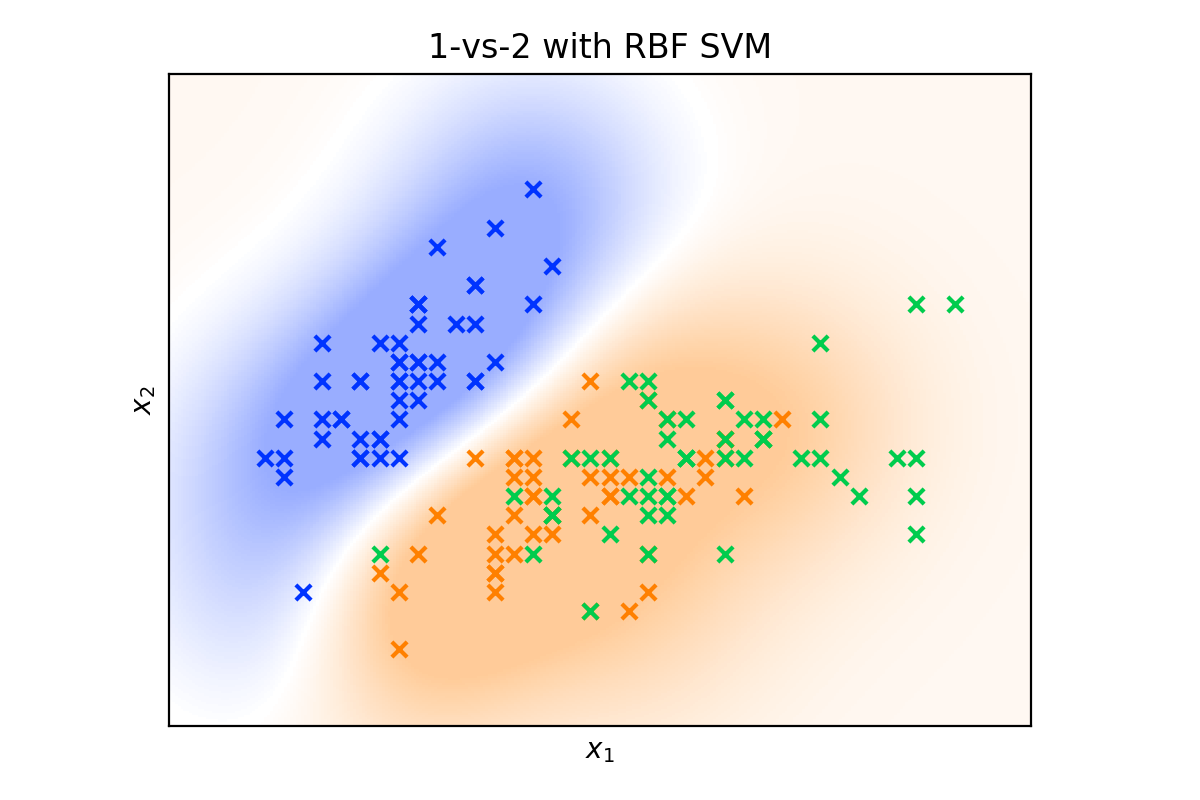
\includegraphics[width=\linewidth]{sample_image.png}
   \end{center}
      \caption{This is the caption of a column-width figure.\label{first_figure}}
\end{figure}
   

% DELETE THIS FIGURE
\begin{figure*}
   \begin{center}
      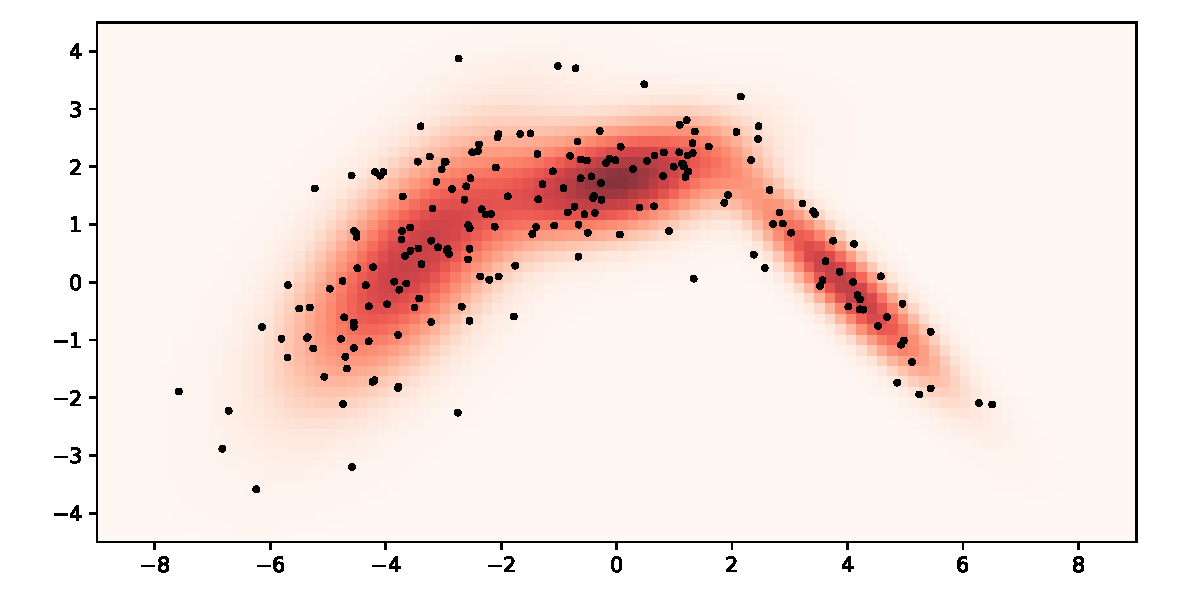
\includegraphics[width=0.4\linewidth]{sample_image.pdf}
      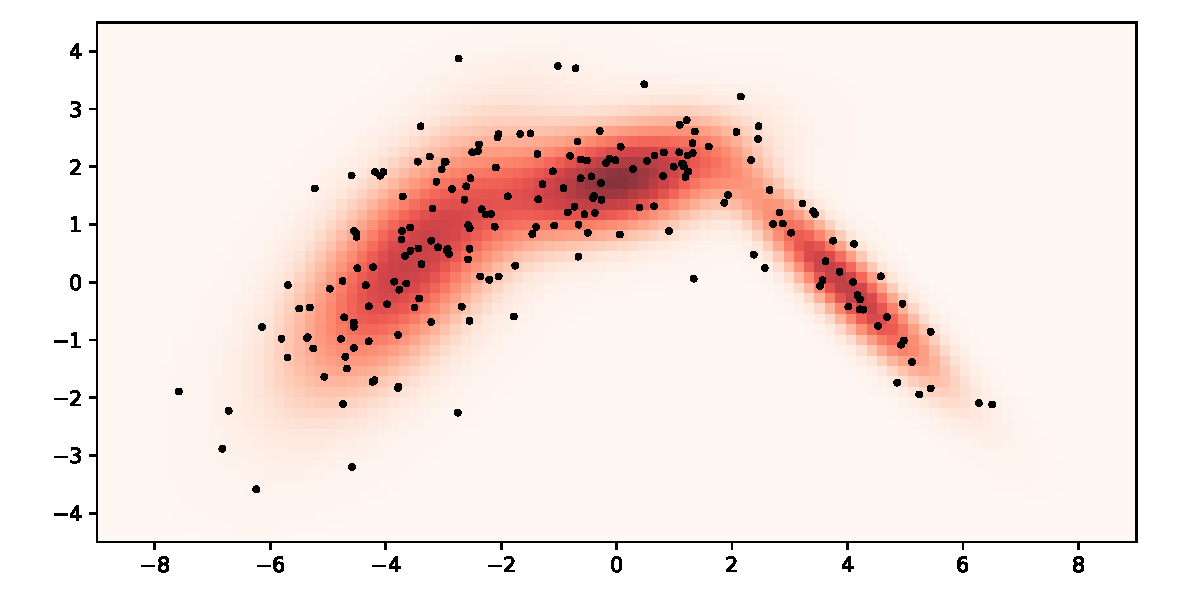
\includegraphics[width=0.4\linewidth]{sample_image.pdf}
   \end{center}
      \caption{This is the caption of a page-width figure.\label{second_figure}}
\end{figure*}





{\small
\bibliographystyle{cvpr_bibstyle}
\bibliography{bibliography}
}

\end{document}
